%%==================================================
%% chapter01.tex for BIT Master Thesis
%% modified by yang yating
%% version: 0.1
%% last update: Dec 25th, 2016

%% modified by Meng Chao
%% version: 0.2
%% last update: May 29th, 2017
%%==================================================
\chapter{绪论}
\label{chap:intro}

\section{论文研究目的与意义}
近年来微小型无人机发展日趋迅速,对无人机导航系统的要求逐步提高,现有的经典导航方法在一些场景中受到限制。例如, GPS 只能用于开阔无遮挡的室外环境,且定位精度不高(非差分)。高精度的惯导系统成本过高难以民用,低成本IMU精度较差,且惯导系统只能估计无人机自身状态,无法感知周围的环境信息。无线信号定位方法需要预先布置使用场景,难以大范围应用。基于机器视觉的定位算法因其硬件成本低廉,精度较高,可感知丰富的环境信息,无需事先布置场景等优势,成为目前无人机定位导航的研究热点。

对于视觉定位而言一个基本而重要的问题是如何通过二维的图像信息分析景物的三维结构,确定相机在其中的位置。经过近30年的长足发展,人们在这个问题上取得了众多令人兴奋的成果,这其中离不开一项基本技术的研究:同步定位与地图重建(Simultaneous Localization and Mapping,SLAM),特别是基于视觉的SLAM技术。同步定位与地图构建技术(下文简称SLAM),旨在解决携带传感器的运动物体,在运动过程中如何对自身进行定位,同时以合适的方式建模周围环境的问题。根据所携传感器的不同,可以把 SLAM分成激光和视觉两大类。激光SLAM在理论和实践上均较为成熟,已较好地应用于机器人等行业。而视觉SLAM则起步较晚,如果把环境限定在光照、纹理充足,由静态的刚体组成的场合,现有的视觉SLAM可以令人满意地运行。而针对实际应用场景,无论从精度、效率、鲁棒性上来说,都与理想的情况相去甚远。

在视觉SLAM算法中,根据所用传感器不同可以分为RGB-D SLAM,双目SLAM和单目SLAM三种。无人机一般运行在大场景和变尺度的环境下,而 RGB-D相机量程有限,噪声大;双目相机受到基线的限制,在景深远大于基线距离时获得的深度误差很大而退化成单目,都无法用于大尺度和变尺度场景中。而单目相机不存在基线与深度测量量程的限制,结构简单,计算效率高,广泛应用于大尺度环境和变尺度场景。

当前的单目SLAM算法很难在保证定位精度和鲁棒性的前提下提供丰富的环境地图;并且由于单目相机无法提供深度信息,得到的运动轨迹和环境地图的尺度不确定,因而无法用于导航和环境感知。本文研究并对比主流单目SLAM算法,对基于特征的单目SLAM算法
进行改进,研究基于概率逆深度估计的单目半稠密SLAM算法,并将惯性测量单元(IMU)与单目进行信息融合。在保证定位精度和鲁棒性的前提下,得到有确定尺度的轨迹和环境半稠密地图,应用于无人机在陌生环境下的定位和导航。
\section{无人机定位技术研究现状}
随着多旋翼无人机的发展,其飞行范围从实验区域扩展到室外丛林,城市和室内生活区。但复杂环境中一般都在噪声干扰、信号遮挡和动态运动目标,这对无人机的导航定位提出了更高的要求。传统的导航定位方法如GPS和惯导系统存在局限,如GPS只能用于室外且对于非差分的GPS定位精度较低。低成本惯导本身存在较大漂移,定位精度差。近年来利用机载传感器(如激光雷达、摄像头或光流等)进行多传感器数据融合逐渐成为无人机定位与导航领域的研究重点。

美国犹他州立大学的四旋翼无人机采用Gumstix的Verdex Pro XL6P芯片,机载传感器为惯性测量元件(IMU)、声纳传感器,单目摄像头,红外探测摄像头等。采用基于视觉图像的SLAM算法进行无人机定位和导航,实现在地面站平台,导航信息通过无线数传发送给无人机,完成无人机的导航和任务规划,还可根据红外探测摄像头对室内物体进行检测。宾夕法尼亚大学选用Ascending Tech-nologies GmbH无人机,使用Intel Atom 1.6 GHz CPU作为控制平台,机上携带激光雷达,摄像机、IMU和两个测高望远镜,采用基于网络搜索的ICP算法利用激光雷达进行定位,利用视觉SLAM矫正位姿误差,并利用扩展卡尔曼滤波(EKF)实现多传感器数据融合。依靠多层次的环境重构、定位、轨迹规划和控制在室内实现全自主飞行,并且对外部环境的变化具有较好的鲁棒性。弗莱堡大学选用Mikrokopter无人机,机上载荷包括激光雷达和航姿系统,采用激光SLAM算法并通过粒子滤波实现多传感器融合,完成在已知或位置环境下的见图与定位、航迹规划和无人机控制。

综上所述,SLAM技术已广泛应用于无人机定位与导航。相比于传统的惯性导航和卫星导航,SLAM技术不受限于室内外场景,定位精度高,结构简单,漂移小,功耗低,鲁棒性好,不需要环境的先验信息,可以满足多旋翼无人机的定位和导航需要。

\section{视觉SLAM国内外研究现状}
\subsection{国外研究现状}
SLAM技术最早始于1985年\upcite{},在1986年至1990年期间,R.Smith提出了SLAM问题并给出了初步的解决方案\upcite{}。他率先以概率形式讨论机器人轨迹与地图之间的不确定性,并将扩展卡尔曼滤波应用在SLAM问题。相比于之前的确定性方法,基于概率形式的方法更灵活、搞笑的表达轨迹与地图的估计,可以在理论上分析、推导SLAM问题的数学表达。这一方法在随后的十几年间成为主流,得到了充分的研究和扩展\upcite{}。主要的研究方向包括:扩展EKF应用场景的规模\upcite{}、解决EKF中的数据关联问题\upcite{}、减少EKF的计算量\upcite{}、使用其他种类的滤波器\upcite{}。

遵循前辈们的轨迹,研究者们在21世纪初期开始了视觉SLAM的研究。与激光传感器不同,视觉传感器的运动天生属于三维空间。不过,图像跟踪的特征点可以看做SLAM的路标点,适用于传统SLAM算法的位姿——路标框架。相比于传统的激光SLAM算法,视觉传感器具有便宜、轻便、信息丰富等多种优点,但是它的特征点数量多,没有距离信息,对算法和硬件设计提出了挑战。2007年,A.J.Davison经过长期的研究,首次实现实时视觉SLAM EKF SLAM系统——MonoSLAM。这具有里程碑的意义,该系统以EKF作为后端,跟踪前端提取的很稀疏的Harris特征点,减少了计算规模,把视觉SLAM算法实时化。

21世纪中,视觉SLAM经历了以上一系列重要的发展,产生了一批现有的视觉SLAM解决方案,如表\ref{tab1.1}所示。SLAM技术的发展可以分理论和算法两个方面。




\begin{table}[h]		%表格环境
% \multicolumn是跨列功能,第一个参数2,表示跨两列,第二个参数c|,表示文字置中,并在栏位右边画一条直线框,最后一个参数即是要填入的文字
%\multirow是跨行功能,第一个参数2,表示跨两行,第二个参数*,表示系统自动调整文字,最后一个参数即是要填入的文字
\newcommand{\tabincell}[2]{\begin{tabular}{@{}#1@{}}#2\end{tabular}}		%单元格内容强制换行
\renewcommand\arraystretch{1.5}		%增加行间距
\centering
\caption{现代代表性SLAM方案}   % 表格标题,在表格内容之前
\label{tab3.1}
	\begin{tabular*}{0.9\textwidth}{@{\extracolsep{\fill}}ccc}  %生成行和列的表格
	
	\end{tabular*}
\end{table}


\section{论文主要内容和结构安排}



\iffalse
\begin{figure}
  \centering
  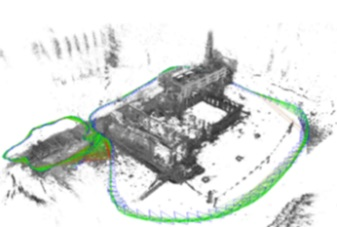
\includegraphics[height=0.5\textwidth]{figures/Fig1(1)}
  %\caption{The UAV equipped with an ASUS Xtion Pro Live RGB-D camera}
  %\label{Figure1.};
  
  \centering
  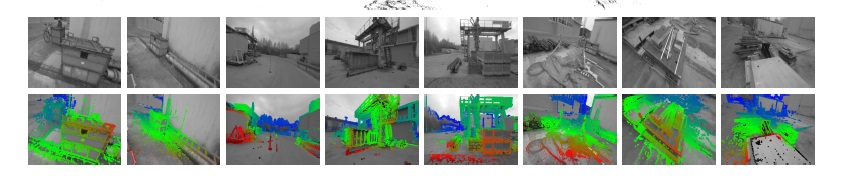
\includegraphics[width=0.75\textwidth]{figures/Fig1(2)}
  \caption{LSD-SLAM generates a consistent global map}
  %\label{referencename};
\end{figure}
\fi
